\documentclass[11pt]{amsart}

\usepackage[
% fancytheorems, 
% fancyproofs,
% noindent, 
nokoma
%spacingfix, 
]{adam}

% \usepackage{ulem}
% \DeclareRobustCommand{\hsout}[1]{\texorpdfstring{\sout{#1}}{#1}}

\usepackage{cancel}
\usepackage{tikz}

% \usepackage{titling}
% \setlength{\droptitle}{-4em}

\newcommand{\op}{\overline{\varphi}}


\title{Quotient Groups \& The Isomorphism Theorem}
% \title{\vspace{-3\baselineskip}\ \\Quotient Groups \& The Isomorphism Theorem}
\author{Adam Kelly (\texttt{ak2316@cam.ac.uk})}
\date{\today}

\begin{document}


\maketitle

Quotient groups arise naturally in the study of homomorphisms. When we have two groups $G$ and $H$, and some homomorphism $\varphi: G \rightarrow H$, we can see that the elements of $G$ mapping to certain elements of $H$ naturally arrange themselves together.

\begin{center}
	


	\tikzset{every picture/.style={line width=0.75pt}} %set default line width to 0.75pt        

	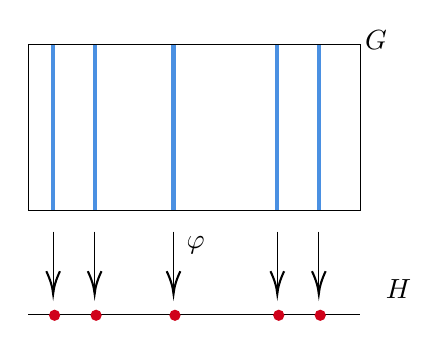
\begin{tikzpicture}[x=0.75pt,y=0.75pt,yscale=-1,xscale=1]
	%uncomment if require: \path (0,300); %set diagram left start at 0, and has height of 300
	
	%Straight Lines [id:da4738114694625044] 
	\draw    (60,170) -- (220,170) ;
	%Straight Lines [id:da11511338342075483] 
	\draw    (130,130) -- (130,158) ;
	\draw [shift={(130,160)}, rotate = 270] [color={rgb, 255:red, 0; green, 0; blue, 0 }  ][line width=0.75]    (10.93,-3.29) .. controls (6.95,-1.4) and (3.31,-0.3) .. (0,0) .. controls (3.31,0.3) and (6.95,1.4) .. (10.93,3.29)   ;
	%Shape: Circle [id:dp33651349641998407] 
	\draw  [draw opacity=0][fill={rgb, 255:red, 208; green, 2; blue, 27 }  ,fill opacity=1 ] (128,170.3) .. controls (128,168.81) and (129.21,167.6) .. (130.7,167.6) .. controls (132.19,167.6) and (133.4,168.81) .. (133.4,170.3) .. controls (133.4,171.79) and (132.19,173) .. (130.7,173) .. controls (129.21,173) and (128,171.79) .. (128,170.3) -- cycle ;
	%Straight Lines [id:da5155967431204146] 
	\draw [color={rgb, 255:red, 74; green, 144; blue, 226 }  ,draw opacity=1 ][line width=1.5]    (130,40) -- (130,120) ;
	%Straight Lines [id:da14331674756217372] 
	\draw    (72,130) -- (72,158) ;
	\draw [shift={(72,160)}, rotate = 270] [color={rgb, 255:red, 0; green, 0; blue, 0 }  ][line width=0.75]    (10.93,-3.29) .. controls (6.95,-1.4) and (3.31,-0.3) .. (0,0) .. controls (3.31,0.3) and (6.95,1.4) .. (10.93,3.29)   ;
	%Shape: Circle [id:dp5096396309384827] 
	\draw  [draw opacity=0][fill={rgb, 255:red, 208; green, 2; blue, 27 }  ,fill opacity=1 ] (70,170.3) .. controls (70,168.81) and (71.21,167.6) .. (72.7,167.6) .. controls (74.19,167.6) and (75.4,168.81) .. (75.4,170.3) .. controls (75.4,171.79) and (74.19,173) .. (72.7,173) .. controls (71.21,173) and (70,171.79) .. (70,170.3) -- cycle ;
	%Straight Lines [id:da9845694947039054] 
	\draw [color={rgb, 255:red, 74; green, 144; blue, 226 }  ,draw opacity=1 ][line width=1.5]    (72,40) -- (72,120) ;
	%Straight Lines [id:da10408362603379395] 
	\draw    (92,130) -- (92,158) ;
	\draw [shift={(92,160)}, rotate = 270] [color={rgb, 255:red, 0; green, 0; blue, 0 }  ][line width=0.75]    (10.93,-3.29) .. controls (6.95,-1.4) and (3.31,-0.3) .. (0,0) .. controls (3.31,0.3) and (6.95,1.4) .. (10.93,3.29)   ;
	%Shape: Circle [id:dp592184874768645] 
	\draw  [draw opacity=0][fill={rgb, 255:red, 208; green, 2; blue, 27 }  ,fill opacity=1 ] (90,170.3) .. controls (90,168.81) and (91.21,167.6) .. (92.7,167.6) .. controls (94.19,167.6) and (95.4,168.81) .. (95.4,170.3) .. controls (95.4,171.79) and (94.19,173) .. (92.7,173) .. controls (91.21,173) and (90,171.79) .. (90,170.3) -- cycle ;
	%Straight Lines [id:da7856952867633485] 
	\draw [color={rgb, 255:red, 74; green, 144; blue, 226 }  ,draw opacity=1 ][line width=1.5]    (92,40) -- (92,120) ;
	%Straight Lines [id:da18609223529659646] 
	\draw    (180,130) -- (180,158) ;
	\draw [shift={(180,160)}, rotate = 270] [color={rgb, 255:red, 0; green, 0; blue, 0 }  ][line width=0.75]    (10.93,-3.29) .. controls (6.95,-1.4) and (3.31,-0.3) .. (0,0) .. controls (3.31,0.3) and (6.95,1.4) .. (10.93,3.29)   ;
	%Straight Lines [id:da005590924400573405] 
	\draw [color={rgb, 255:red, 74; green, 144; blue, 226 }  ,draw opacity=1 ][line width=1.5]    (180,40) -- (180,120) ;
	%Straight Lines [id:da8680905965357972] 
	\draw    (200,130) -- (200,158) ;
	\draw [shift={(200,160)}, rotate = 270] [color={rgb, 255:red, 0; green, 0; blue, 0 }  ][line width=0.75]    (10.93,-3.29) .. controls (6.95,-1.4) and (3.31,-0.3) .. (0,0) .. controls (3.31,0.3) and (6.95,1.4) .. (10.93,3.29)   ;
	%Straight Lines [id:da5630035947767571] 
	\draw [color={rgb, 255:red, 74; green, 144; blue, 226 }  ,draw opacity=1 ][line width=1.5]    (200,40) -- (200,120) ;
	%Shape: Rectangle [id:dp9314276081609332] 
	\draw   (60,40) -- (220,40) -- (220,120) -- (60,120) -- cycle ;
	%Shape: Circle [id:dp7562554584334911] 
	\draw  [draw opacity=0][fill={rgb, 255:red, 208; green, 2; blue, 27 }  ,fill opacity=1 ] (178,170.3) .. controls (178,168.81) and (179.21,167.6) .. (180.7,167.6) .. controls (182.19,167.6) and (183.4,168.81) .. (183.4,170.3) .. controls (183.4,171.79) and (182.19,173) .. (180.7,173) .. controls (179.21,173) and (178,171.79) .. (178,170.3) -- cycle ;
	%Shape: Circle [id:dp9004298600298029] 
	\draw  [draw opacity=0][fill={rgb, 255:red, 208; green, 2; blue, 27 }  ,fill opacity=1 ] (198,170.3) .. controls (198,168.81) and (199.21,167.6) .. (200.7,167.6) .. controls (202.19,167.6) and (203.4,168.81) .. (203.4,170.3) .. controls (203.4,171.79) and (202.19,173) .. (200.7,173) .. controls (199.21,173) and (198,171.79) .. (198,170.3) -- cycle ;
	
	% Text Node
	\draw (221,32) node [anchor=north west][inner sep=0.75pt]    {$G$};
	% Text Node
	\draw (231,152) node [anchor=north west][inner sep=0.75pt]    {$H$};
	% Text Node
	\draw (135,131) node [anchor=north west][inner sep=0.75pt]    {$\varphi $};
	% Text Node
	\draw (100,80) node [anchor=north west][inner sep=0.75pt]    {$\dotsc $};
	% Text Node
	\draw (145,80) node [anchor=north west][inner sep=0.75pt]    {$\dotsc $};
	
	
	\end{tikzpicture}
	
\end{center}


Indeed, if two elements of $G$ map to the same element of $H$ under $\varphi$, we would find that the two elements must differ by an element of the kernel of $\varphi$. So, going back to how the elements of $G$ arrange themselves, it would seem that they are arranged into cosets of the kernel of $\varphi$. It is this observation that leads us to the definition of quotient groups and the isomorphism theorems.


From the discussion above, it is natural to see when we can make the cosets of a given subgroup into another group. It turns out that this only works when we have a specific type of subgroup.

\begin{definition*}[Normal Subgroup]
	We say that a subgroup $N$ of a group $G$ is \vocab{normal} if the left and right cosets coincide, that is, $gN = Ng$ for all $g \in G$. If $N$ is normal in $G$ we write $N \normal G$.
\end{definition*}

Now we can show that the set of cosets of $N$ in $G$, written $G/N$, forms a group.

\begin{theorem*}[Quotient Groups]
	If $N \normal G$, then the set of cosets of $N$ in $G$ forms the \vocab{quotient group} $G/N$ with the operation of coset multiplication, where $gN \cdot g'N = (g g')N$.
\end{theorem*}
\begin{proof}
	We first need to check that coset multiplication is well defined. If we had $a_1 N = a_2N$ and $b_1 N = b_2 N$, then $a_1 = a_2 n_a$ and $b_1 = b_2 n_b$ for some $n_a, n_b \in N$. Then $(a_1 b_1)N = (a_2 n_a b_2 n_b)N = (a_2 b_2)N$, since $N$ is normal in $G$. So our group operation is well defined, and we are just left to check the group axioms.

	We have closure since $g_1 N$ and $g_2N$ being cosets implies $(g_1 g_2)N$ is too. Then we have the identity element $N$, and inverses with $gN \cdot g^{-1}N = N$. Finally we get associativity inherited from $G$, thus we do indeed have a group.
\end{proof}

Now we initially tried to motivate thinking about groups of cosets by noticing that elements in the same coset of the kernel of $\phi$ had the same image. We then used this `normal' property of a subgroup to make this actually work. It turns out that these express the same idea -- normal subgroups are \emph{exactly} the kernels of homomorphisms.

\begin{theorem*}[Kernels are Normal Subgroups]
	If $\phi: G \rightarrow H$ is a homomorphism, then $\ker \phi \normal G$.
\end{theorem*}
\begin{proof}
	We already know that the kernel of a homomorphism is a subgroup, so we just need to check that it is normal. Let $n \in \ker \phi$, and $g \in G$. Then $\phi(gng^{-1}) = \phi(g) \phi(n)\phi(g^{-1}) = \phi(g) \phi(g^{-1}) = e$, thus $gng^{-1} \in \ker \phi$, so $\ker \phi \normal G$ as required.
\end{proof}

\begin{theorem*}[Normal Subgroups are Kernels]
	Given $N \normal G$, the map $\pi: G \mapsto G/N$ with $\pi(g) = gN$ is a surjective homomorphism called the \vocab{quotient map}, and $\kernel \pi = N$. 
\end{theorem*}
\begin{proof}
We first check that $\pi$ is a homomorphism. For $g, h \in G$, we have $\pi(gh) = (gh)N = gN \cdot hN = \pi(g) \pi(h)$ as required. This map is clearly injective, and also $\pi(g) = gN = N \iff g \in N$, so $\ker \pi = N$, as required.
\end{proof}


Looking back again to our original motivation, we can see that the cosets of the kernel seem to form the group that is the image of the homomorphism. This is the exact idea encompassed in quotient groups, and is formalised in the \emph{first isomorphism theorem}.

\begin{theorem*}[First Isomorphism Theorem]
	Let $\varphi:G \rightarrow H$ be a homomorphism. Then $G/\kernel \varphi \cong \image \varphi$.
\end{theorem*}
\begin{proof}
	Consider the map $\op: G/\ker\varphi \rightarrow \image \varphi$ with $g\ker\varphi \mapsto \varphi(g)$. It's easy to see that this is well defined and to check that it's a homomorphism. It's also clearly bijective, and is thus an isomorphism.
\end{proof}

In a sense, this is the way that you should think about normal subgroups and quotient groups -- as the kernels and images of homomorphisms.

\end{document}

% Citations: 

% This page for counterexample 
% https://math.stackexchange.com/questions/2333666/group-is-isomorphic-to-direct-product-of-its-subgroups
